\documentclass[border=6pt]{standalone}
\usepackage[T1]{fontenc}
\usepackage[utf8]{inputenc}
\usepackage[scaled=0.98]{helvet}
\renewcommand{\familydefault}{\sfdefault}
\usepackage{amsmath}
\usepackage{graphicx}
\graphicspath{{../../../../../../exercises_lecturenotes/lecture_notes/kurs100_lektionsnoter/}}
\usepackage{tikz}
\usepackage{pgfplots}
\pgfplotsset{compat=1.18}
\usetikzlibrary{arrows.meta, decorations.pathreplacing, calc, positioning, fit, backgrounds, shapes.geometric}
\usepgfplotslibrary{groupplots,fillbetween}
\definecolor{scanpink}{HTML}{E5006D}
\definecolor{scanteal}{HTML}{00A6A6}
\definecolor{scannavy}{HTML}{243746}
\definecolor{scanlightgray}{HTML}{F1F2F3}
\begin{document}
  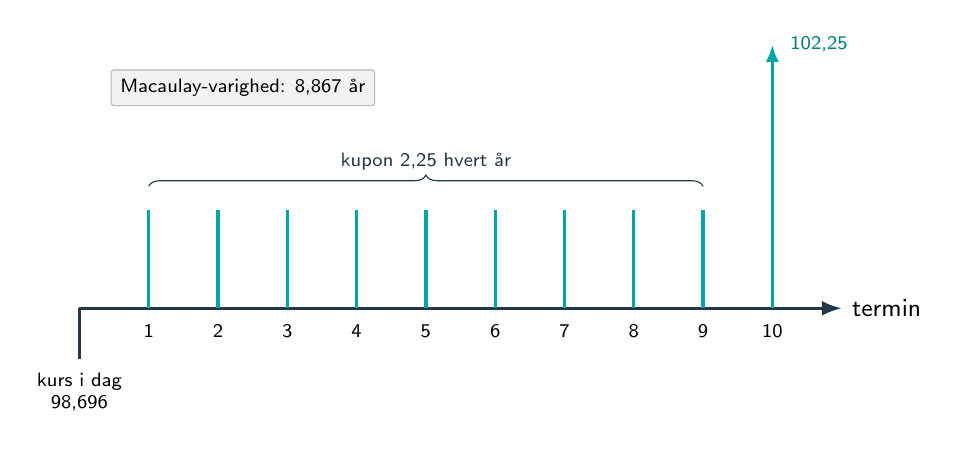
\begin{tikzpicture}[
      x=0.88cm,
      y=1cm,
      font=\small,
      timeline/.style={-{Latex[length=2.5mm]}, line width=0.9pt, draw=scannavy},
      payment/.style={line width=1.2pt, draw=scanteal}
  ]
    \draw[timeline] (0,0) -- (11,0) node[right] {termin};
    \foreach \x in {1,...,9} {
      \draw[payment] (\x,0) -- (\x,1.25);
      \node[font=\scriptsize, anchor=north] at (\x,-0.08) {\x};
    }
    \draw[payment, -{Latex[length=2.2mm]}] (10,0) -- (10,3.35);
    \node[font=\scriptsize, anchor=north] at (10,-0.08) {10};
    \draw[decorate, decoration={brace, amplitude=4pt}, scannavy]
      (1,1.55) -- (9,1.55)
      node[midway, yshift=9pt, font=\scriptsize] {kupon 2,25 hvert år};
    \node[font=\scriptsize, scanteal!75!black, anchor=west] at (10.12,3.35)
      {102,25};
    \draw[scannavy, line width=0.8pt] (0,0) -- (0,-0.65);
    \node[font=\scriptsize, anchor=north, align=center] at (0,-0.7)
      {kurs i dag\\98,696};
    \node[draw=scannavy!35, fill=scanlightgray, rounded corners=1pt,
          font=\scriptsize, anchor=west] at (0.45,2.8)
          {Macaulay-varighed: 8,867 år};
  \end{tikzpicture}
\end{document}
